\documentclass[12pt,a4paper]{article}

\usepackage{amsmath}
\usepackage{amssymb}
\usepackage{geometry}
\usepackage{tikz}
\usepackage{array}
\usepackage{enumitem}

\geometry{margin=1in}
\raggedbottom

\begin{document}

\begin{center}
    {\LARGE\textbf{Height Balanced Trees}}
\end{center}

\vspace{0.5cm}

\section{Skewed Binary Search Tree}



Consider the keys

\[
[3,6,8,10,11,15,20,35]
\]

inserted into a BST in the given order.

Since the keys are inserted in increasing order, the resulting BST is skewed to the right.

\begin{center}
\begin{tikzpicture}[
    every node/.style={circle, draw, minimum size=7mm}
]
\node (n3) at (0,0) {3};
\node (n6) at (1,-1) {6};
\node (n8) at (2,-2) {8};
\node (n10) at (3,-3) {10};
\node (n11) at (4,-4) {11};
\node (n15) at (5,-5) {15};
\node (n20) at (6,-6) {20};
\node (n35) at (7,-7) {35};

\draw[-latex] (n3) -- (n6);
\draw[-latex] (n6) -- (n8);
\draw[-latex] (n8) -- (n10);
\draw[-latex] (n10) -- (n11);
\draw[-latex] (n11) -- (n15);
\draw[-latex] (n15) -- (n20);
\draw[-latex] (n20) -- (n35);
\end{tikzpicture}
\end{center}

The height of this tree is $O(n)$, which makes searching, insertion, and deletion potentially take $O(n)$ time.

\section{AVL Tree}

An AVL tree is a self-balancing Binary Search Tree in which the heights of the left and right subtrees of every node differ by at most one.

The balance factor of a node is defined as

\[
BF = h(\text{left subtree}) - h(\text{right subtree})
\]

For an AVL tree,

\[
BF \in \{-1,0,+1\}
\]

for every node.

If the balance factor becomes less than $-1$ or greater than $+1$, rotations are performed to restore the balance.

The four types of AVL rotations are:

\begin{enumerate}
    \item Left Rotation
    \item Right Rotation
    \item Left-Right Rotation
    \item Right-Left Rotation
\end{enumerate}

An AVL tree has height

\[
O(\log n)
\]

Therefore, search, insertion, and deletion take

\[
O(\log n)
\]

time.

\section{Height Adjustment of the Given BST}

The original BST is highly skewed. To make it height balanced, AVL rotations are performed during insertion.

For the keys

\[
[3,6,8,10,11,15,20,35]
\]

the resulting AVL tree is:

\begin{center}
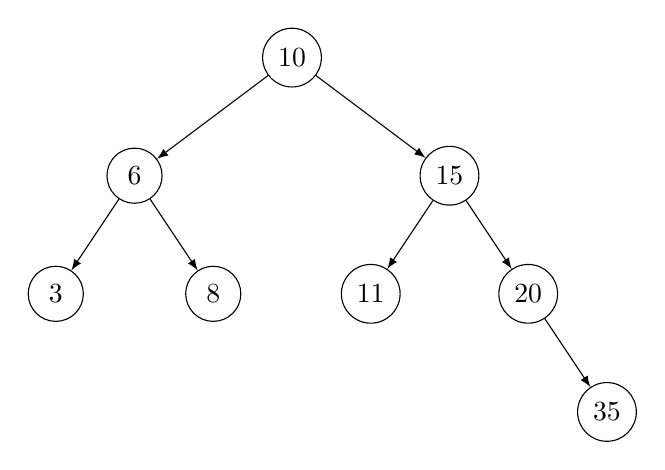
\begin{tikzpicture}[
    every node/.style={circle, draw, minimum size=7mm}
]
\node (n10) at (0,3) {10};
\node (n6) at (-2,1.5) {6};
\node (n15) at (2,1.5) {15};
\node (n3) at (-3,0) {3};
\node (n8) at (-1,0) {8};
\node (n11) at (1,0) {11};
\node (n20) at (3,0) {20};
\node (n35) at (4,-1.5) {35};

\draw[-latex] (n10) -- (n6);
\draw[-latex] (n10) -- (n15);
\draw[-latex] (n6) -- (n3);
\draw[-latex] (n6) -- (n8);
\draw[-latex] (n15) -- (n11);
\draw[-latex] (n15) -- (n20);
\draw[-latex] (n20) -- (n35);
\end{tikzpicture}
\end{center}

For every node in this tree, the balance factor is within

\[
[-1,+1].
\]

Therefore, the tree satisfies the AVL height-balance condition.

\section{Red-Black Tree}

A Red-Black Tree is a self-balancing Binary Search Tree in which every node has a color: red or black.

A Red-Black Tree satisfies the following conditions:

\begin{enumerate}
    \item Every node is either red or black.
    \item The root is black.
    \item Every NIL leaf is black.
    \item A red node cannot have a red child.
    \item Every path from a node to its descendant NIL leaves contains the same number of black nodes.
\end{enumerate}

These conditions ensure that the tree remains approximately balanced.

The height of a Red-Black Tree is

\[
O(\log n).
\]

Therefore, search, insertion, and deletion take

\[
O(\log n)
\]

time.

\section{Deletion from the Height-Balanced Tree}

We now delete the keys

\[
6,\quad 11,\quad 20
\]

from the AVL tree while maintaining the AVL balance condition.

\subsection{Deletion of 6}

Before deletion:

\begin{center}
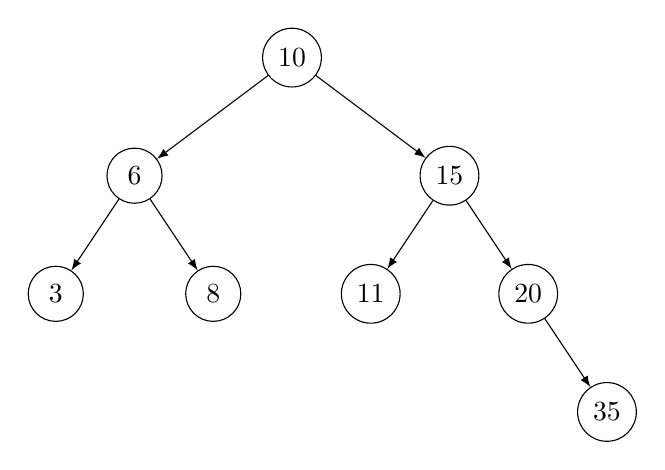
\begin{tikzpicture}[
    every node/.style={circle, draw, minimum size=7mm}
]
\node (n10) at (0,3) {10};
\node (n6) at (-2,1.5) {6};
\node (n15) at (2,1.5) {15};
\node (n3) at (-3,0) {3};
\node (n8) at (-1,0) {8};
\node (n11) at (1,0) {11};
\node (n20) at (3,0) {20};
\node (n35) at (4,-1.5) {35};

\draw[-latex] (n10) -- (n6);
\draw[-latex] (n10) -- (n15);
\draw[-latex] (n6) -- (n3);
\draw[-latex] (n6) -- (n8);
\draw[-latex] (n15) -- (n11);
\draw[-latex] (n15) -- (n20);
\draw[-latex] (n20) -- (n35);
\end{tikzpicture}
\end{center}

Node $6$ has two children, $3$ and $8$.

Using the in-order successor, $8$ replaces $6$.

The resulting tree is:

\begin{center}
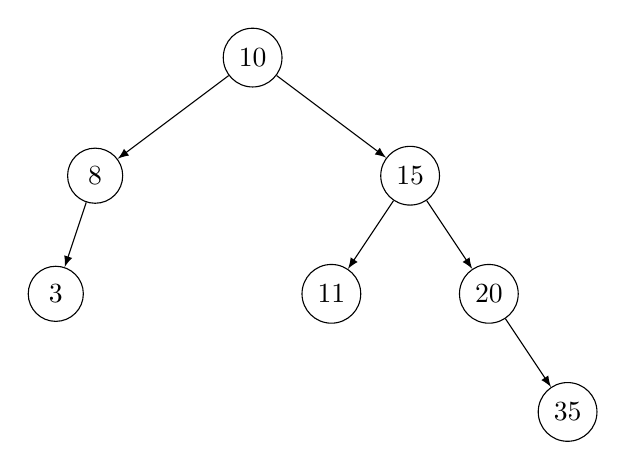
\begin{tikzpicture}[
    every node/.style={circle, draw, minimum size=7mm}
]
\node (n10) at (0,3) {10};
\node (n8) at (-2,1.5) {8};
\node (n15) at (2,1.5) {15};
\node (n3) at (-2.5,0) {3};
\node (n11) at (1,0) {11};
\node (n20) at (3,0) {20};
\node (n35) at (4,-1.5) {35};

\draw[-latex] (n10) -- (n8);
\draw[-latex] (n10) -- (n15);
\draw[-latex] (n8) -- (n3);
\draw[-latex] (n15) -- (n11);
\draw[-latex] (n15) -- (n20);
\draw[-latex] (n20) -- (n35);
\end{tikzpicture}
\end{center}

The balance factors remain within the required range, so no rotation is required.

\subsection{Deletion of 11}

Before deletion, the tree is:

\begin{center}
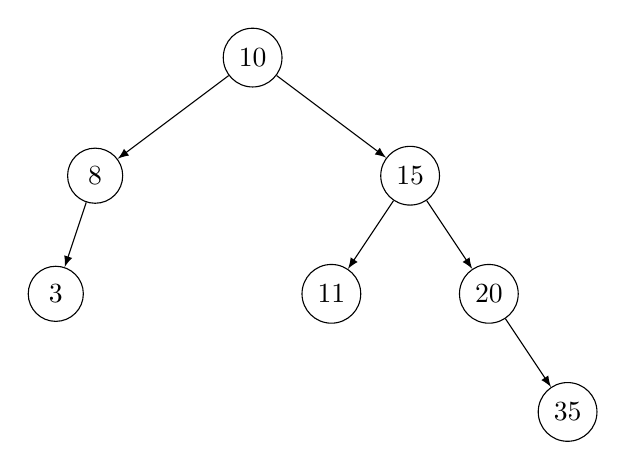
\begin{tikzpicture}[
    every node/.style={circle, draw, minimum size=7mm}
]
\node (n10) at (0,3) {10};
\node (n8) at (-2,1.5) {8};
\node (n15) at (2,1.5) {15};
\node (n3) at (-2.5,0) {3};
\node (n11) at (1,0) {11};
\node (n20) at (3,0) {20};
\node (n35) at (4,-1.5) {35};

\draw[-latex] (n10) -- (n8);
\draw[-latex] (n10) -- (n15);
\draw[-latex] (n8) -- (n3);
\draw[-latex] (n15) -- (n11);
\draw[-latex] (n15) -- (n20);
\draw[-latex] (n20) -- (n35);
\end{tikzpicture}
\end{center}

Node $11$ is a leaf, so it is simply removed.

The resulting tree is:

\begin{center}
\begin{tikzpicture}[
    every node/.style={circle, draw, minimum size=7mm}
]
\node (n10) at (0,3) {10};
\node (n8) at (-2,1.5) {8};
\node (n15) at (2,1.5) {15};
\node (n3) at (-2.5,0) {3};
\node (n20) at (2,0) {20};
\node (n35) at (3,-1.5) {35};

\draw[-latex] (n10) -- (n8);
\draw[-latex] (n10) -- (n15);
\draw[-latex] (n8) -- (n3);
\draw[-latex] (n15) -- (n20);
\draw[-latex] (n20) -- (n35);
\end{tikzpicture}
\end{center}

The balance factors remain within

\[
[-1,+1],
\]

so no rotation is required.

\subsection{Deletion of 20}

Before deletion, the tree is:

\begin{center}
\begin{tikzpicture}[
    every node/.style={circle, draw, minimum size=7mm}
]
\node (n10) at (0,3) {10};
\node (n8) at (-2,1.5) {8};
\node (n15) at (2,1.5) {15};
\node (n3) at (-2.5,0) {3};
\node (n20) at (2,0) {20};
\node (n35) at (3,-1.5) {35};

\draw[-latex] (n10) -- (n8);
\draw[-latex] (n10) -- (n15);
\draw[-latex] (n8) -- (n3);
\draw[-latex] (n15) -- (n20);
\draw[-latex] (n20) -- (n35);
\end{tikzpicture}
\end{center}

Node $20$ has one child, $35$. Therefore, $35$ replaces $20$.

The resulting tree is:

\begin{center}
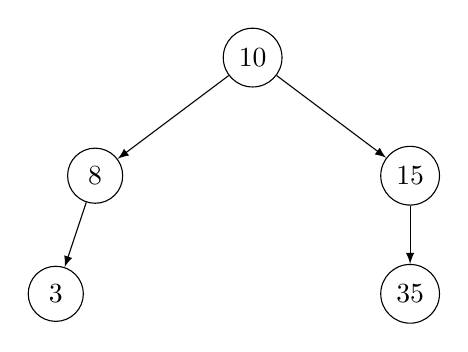
\begin{tikzpicture}[
    every node/.style={circle, draw, minimum size=7mm}
]
\node (n10) at (0,3) {10};
\node (n8) at (-2,1.5) {8};
\node (n15) at (2,1.5) {15};
\node (n3) at (-2.5,0) {3};
\node (n35) at (2,0) {35};

\draw[-latex] (n10) -- (n8);
\draw[-latex] (n10) -- (n15);
\draw[-latex] (n8) -- (n3);
\draw[-latex] (n15) -- (n35);
\end{tikzpicture}
\end{center}

The final AVL tree is balanced because every node has a balance factor in

\[
\{-1,0,+1\}.
\]

The remaining keys are

\[
[3,8,10,15,35].
\]

\section{B-Tree}

A B-Tree is a self-balancing multiway search tree in which a node can contain multiple keys and multiple children.

For a B-Tree with minimum degree $t$:

\begin{itemize}
    \item A node can contain at most $2t-1$ keys.
    \item A node can have at most $2t$ children.
    \item Every non-root node contains at least $t-1$ keys.
    \item An internal node containing $k$ keys has $k+1$ children.
    \item All leaf nodes are at the same level.
    \item Keys within a node are stored in sorted order.
\end{itemize}

B-Trees remain balanced after insertion and deletion.

The height of a B-Tree is

\[
O(\log n).
\]

B-Trees are commonly used in databases and file systems because a single node can contain many keys, reducing the number of disk accesses.

\section{B+ Tree}

A B+ Tree is a variation of the B-Tree designed for efficient storage and retrieval.

The main properties of a B+ Tree are:

\begin{itemize}
    \item Internal nodes contain keys used for navigation.
    \item Actual records or data pointers are stored only in the leaf nodes.
    \item All leaf nodes are at the same level.
    \item Leaf nodes are linked together.
    \item Keys in the leaf nodes are stored in sorted order.
\end{itemize}

Since the leaf nodes are linked, sequential access and range queries can be performed efficiently.

The height of a B+ Tree is

\[
O(\log n).
\]

B+ Trees are widely used in database indexing and file systems.

\section{B-Tree and B+ Tree Comparison}

\begin{center}
\begin{tabular}{|p{4cm}|p{4cm}|p{4cm}|}
\hline
\textbf{Feature} & \textbf{B-Tree} & \textbf{B+ Tree} \\
\hline
Data storage & Data can be stored in internal and leaf nodes & Data is stored only in leaf nodes \\
\hline
Internal nodes & Store keys and possibly data & Store only keys for navigation \\
\hline
Leaf nodes & Not necessarily linked & Linked together \\
\hline
Sequential access & Less efficient & More efficient \\
\hline
Range queries & Efficient & Very efficient \\
\hline
Common use & Databases and file systems & Database indexing and file systems \\
\hline
\end{tabular}
\end{center}

\end{document}

